% Options for packages loaded elsewhere
\PassOptionsToPackage{unicode}{hyperref}
\PassOptionsToPackage{hyphens}{url}
%
\documentclass[
]{book}
\usepackage{amsmath,amssymb}
\usepackage{lmodern}
\usepackage{iftex}
\ifPDFTeX
  \usepackage[T1]{fontenc}
  \usepackage[utf8]{inputenc}
  \usepackage{textcomp} % provide euro and other symbols
\else % if luatex or xetex
  \usepackage{unicode-math}
  \defaultfontfeatures{Scale=MatchLowercase}
  \defaultfontfeatures[\rmfamily]{Ligatures=TeX,Scale=1}
\fi
% Use upquote if available, for straight quotes in verbatim environments
\IfFileExists{upquote.sty}{\usepackage{upquote}}{}
\IfFileExists{microtype.sty}{% use microtype if available
  \usepackage[]{microtype}
  \UseMicrotypeSet[protrusion]{basicmath} % disable protrusion for tt fonts
}{}
\makeatletter
\@ifundefined{KOMAClassName}{% if non-KOMA class
  \IfFileExists{parskip.sty}{%
    \usepackage{parskip}
  }{% else
    \setlength{\parindent}{0pt}
    \setlength{\parskip}{6pt plus 2pt minus 1pt}}
}{% if KOMA class
  \KOMAoptions{parskip=half}}
\makeatother
\usepackage{xcolor}
\usepackage{color}
\usepackage{fancyvrb}
\newcommand{\VerbBar}{|}
\newcommand{\VERB}{\Verb[commandchars=\\\{\}]}
\DefineVerbatimEnvironment{Highlighting}{Verbatim}{commandchars=\\\{\}}
% Add ',fontsize=\small' for more characters per line
\usepackage{framed}
\definecolor{shadecolor}{RGB}{248,248,248}
\newenvironment{Shaded}{\begin{snugshade}}{\end{snugshade}}
\newcommand{\AlertTok}[1]{\textcolor[rgb]{0.94,0.16,0.16}{#1}}
\newcommand{\AnnotationTok}[1]{\textcolor[rgb]{0.56,0.35,0.01}{\textbf{\textit{#1}}}}
\newcommand{\AttributeTok}[1]{\textcolor[rgb]{0.77,0.63,0.00}{#1}}
\newcommand{\BaseNTok}[1]{\textcolor[rgb]{0.00,0.00,0.81}{#1}}
\newcommand{\BuiltInTok}[1]{#1}
\newcommand{\CharTok}[1]{\textcolor[rgb]{0.31,0.60,0.02}{#1}}
\newcommand{\CommentTok}[1]{\textcolor[rgb]{0.56,0.35,0.01}{\textit{#1}}}
\newcommand{\CommentVarTok}[1]{\textcolor[rgb]{0.56,0.35,0.01}{\textbf{\textit{#1}}}}
\newcommand{\ConstantTok}[1]{\textcolor[rgb]{0.00,0.00,0.00}{#1}}
\newcommand{\ControlFlowTok}[1]{\textcolor[rgb]{0.13,0.29,0.53}{\textbf{#1}}}
\newcommand{\DataTypeTok}[1]{\textcolor[rgb]{0.13,0.29,0.53}{#1}}
\newcommand{\DecValTok}[1]{\textcolor[rgb]{0.00,0.00,0.81}{#1}}
\newcommand{\DocumentationTok}[1]{\textcolor[rgb]{0.56,0.35,0.01}{\textbf{\textit{#1}}}}
\newcommand{\ErrorTok}[1]{\textcolor[rgb]{0.64,0.00,0.00}{\textbf{#1}}}
\newcommand{\ExtensionTok}[1]{#1}
\newcommand{\FloatTok}[1]{\textcolor[rgb]{0.00,0.00,0.81}{#1}}
\newcommand{\FunctionTok}[1]{\textcolor[rgb]{0.00,0.00,0.00}{#1}}
\newcommand{\ImportTok}[1]{#1}
\newcommand{\InformationTok}[1]{\textcolor[rgb]{0.56,0.35,0.01}{\textbf{\textit{#1}}}}
\newcommand{\KeywordTok}[1]{\textcolor[rgb]{0.13,0.29,0.53}{\textbf{#1}}}
\newcommand{\NormalTok}[1]{#1}
\newcommand{\OperatorTok}[1]{\textcolor[rgb]{0.81,0.36,0.00}{\textbf{#1}}}
\newcommand{\OtherTok}[1]{\textcolor[rgb]{0.56,0.35,0.01}{#1}}
\newcommand{\PreprocessorTok}[1]{\textcolor[rgb]{0.56,0.35,0.01}{\textit{#1}}}
\newcommand{\RegionMarkerTok}[1]{#1}
\newcommand{\SpecialCharTok}[1]{\textcolor[rgb]{0.00,0.00,0.00}{#1}}
\newcommand{\SpecialStringTok}[1]{\textcolor[rgb]{0.31,0.60,0.02}{#1}}
\newcommand{\StringTok}[1]{\textcolor[rgb]{0.31,0.60,0.02}{#1}}
\newcommand{\VariableTok}[1]{\textcolor[rgb]{0.00,0.00,0.00}{#1}}
\newcommand{\VerbatimStringTok}[1]{\textcolor[rgb]{0.31,0.60,0.02}{#1}}
\newcommand{\WarningTok}[1]{\textcolor[rgb]{0.56,0.35,0.01}{\textbf{\textit{#1}}}}
\usepackage{longtable,booktabs,array}
\usepackage{calc} % for calculating minipage widths
% Correct order of tables after \paragraph or \subparagraph
\usepackage{etoolbox}
\makeatletter
\patchcmd\longtable{\par}{\if@noskipsec\mbox{}\fi\par}{}{}
\makeatother
% Allow footnotes in longtable head/foot
\IfFileExists{footnotehyper.sty}{\usepackage{footnotehyper}}{\usepackage{footnote}}
\makesavenoteenv{longtable}
\usepackage{graphicx}
\makeatletter
\def\maxwidth{\ifdim\Gin@nat@width>\linewidth\linewidth\else\Gin@nat@width\fi}
\def\maxheight{\ifdim\Gin@nat@height>\textheight\textheight\else\Gin@nat@height\fi}
\makeatother
% Scale images if necessary, so that they will not overflow the page
% margins by default, and it is still possible to overwrite the defaults
% using explicit options in \includegraphics[width, height, ...]{}
\setkeys{Gin}{width=\maxwidth,height=\maxheight,keepaspectratio}
% Set default figure placement to htbp
\makeatletter
\def\fps@figure{htbp}
\makeatother
\setlength{\emergencystretch}{3em} % prevent overfull lines
\providecommand{\tightlist}{%
  \setlength{\itemsep}{0pt}\setlength{\parskip}{0pt}}
\setcounter{secnumdepth}{5}
\usepackage{booktabs}
\ifLuaTeX
  \usepackage{selnolig}  % disable illegal ligatures
\fi
\usepackage[]{natbib}
\bibliographystyle{apalike}
\IfFileExists{bookmark.sty}{\usepackage{bookmark}}{\usepackage{hyperref}}
\IfFileExists{xurl.sty}{\usepackage{xurl}}{} % add URL line breaks if available
\urlstyle{same} % disable monospaced font for URLs
\hypersetup{
  pdftitle={Cookbook for CICD with R and GitHub Actions},
  pdfauthor={Yann Say},
  hidelinks,
  pdfcreator={LaTeX via pandoc}}

\title{Cookbook for CICD with R and GitHub Actions}
\author{Yann Say}
\date{2022-12-05}

\begin{document}
\maketitle

{
\setcounter{tocdepth}{1}
\tableofcontents
}
\hypertarget{intro}{%
\chapter{Intro}\label{intro}}

This is a small collections of step-by-step on how to set-up of r-lib GitHub Actions for CICD with R programming. It mainly use the package \texttt{usethis}(version 2.1.6). More details of the actions can be found \href{https://github.com/r-lib/actions/tree/v2-branch/examples}{here}. When I thought necessary I have added a few additional steps, e.g.~when using other services from GitHub or Codecov which I thought was missing when I was trying to learn about GitHub Actions.

The book was built with \href{https://github.com/rstudio/bookdown}{\textbf{bookdown}}.

\hypertarget{r-cmd-check}{%
\chapter{R CMD check}\label{r-cmd-check}}

\hypertarget{r-cmd-check-1}{%
\section{R-CMD-check}\label{r-cmd-check-1}}

Quick how-to to set a github action for a R CMD check each time there is merge into the \textbf{main} (or \textbf{master}) branch using \texttt{r-lib} \href{https://github.com/r-lib/actions/blob/v2-branch/examples/check-release.yaml}{check-release.yaml} or \href{https://github.com/r-lib/actions/blob/v2-branch/examples/check-standard.yaml}{check-standard.yaml}.

\hypertarget{prerequisite}{%
\section{Prerequisite}\label{prerequisite}}

None in particular but could be good to have some \href{https://r-pkgs.org/testing-basics.html}{tests} already.

\hypertarget{steps}{%
\section{Steps}\label{steps}}

\begin{itemize}
\item
  Create your package.
\item
  Try to test your package \texttt{devtools::test()} or \texttt{devtools::check()}

  \begin{itemize}
  \tightlist
  \item
    While this step is not really necessary, it is to make sure your tests runs once and any further problems do not come from the tests.
  \end{itemize}
\item
  Add the check-release.yaml \texttt{usethis::use\_github\_action("check-release")} or check-standard.yaml \texttt{usethis::use\_github\_action("check-standard")}

  \begin{itemize}
  \tightlist
  \item
    check-release.yaml will run R CMD check on Ubuntu and current R version
  \item
    check-standard.yaml will run R CMD check on 3 OS: mac and Windows with the current R version, Ubuntu with the current, development and previous version of R. This what you would want for CRAN.
  \end{itemize}
\item
  Add the badge with \texttt{usethis::use\_github\_actions\_badge("check-release")} or \texttt{usethis::use\_github\_actions\_badge("check-standard")}
\item
  Push!
\end{itemize}

\hypertarget{test-coverage}{%
\chapter{Test coverage}\label{test-coverage}}

\hypertarget{test-coverage-1}{%
\section{test-coverage}\label{test-coverage-1}}

Quick how-to to set a GitHub action to get code coverage and the badge from Codecov each time there is merge into the \textbf{main} (or \textbf{master}) branch using \texttt{r-lib} \href{https://github.com/r-lib/actions/blob/v2-branch/examples/test-coverage.yaml}{test-coverage.yaml}.

\hypertarget{prerequisite-1}{%
\section{Prerequisite}\label{prerequisite-1}}

Have a \href{https://app.codecov.io/}{Codecov} account link with your repository.

None in particular but could be good to have some \href{https://r-pkgs.org/testing-basics.html}{tests} as to get a coverage of something.

\hypertarget{steps-1}{%
\section{Steps}\label{steps-1}}

\begin{itemize}
\item
  Create your package.
\item
  Link your local to the remote if it has not be done yet (make sure your project is linked to a Github repository).
\item
  Make sure Codecov has synced with your repository. The repository should appear in the \emph{Not yet setup} if this is the first time. The syncing between GitHub and Codecov takes a bit of time so you can go for a coffee or lunch.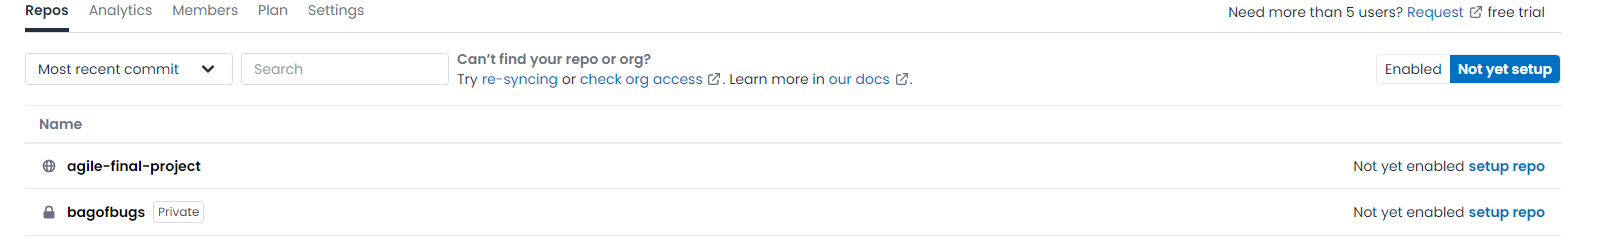
\includegraphics{images/test-coverage/codecovnotyetsetup.png}
\item
  Try to test your package \texttt{covr::package\_coverage()}.

  \begin{itemize}
  \tightlist
  \item
    While this step is not really necessary, it is to make sure your tests runs once and any further problems do not come from the tests.
  \end{itemize}
\item
  Add the test-coverage.yaml \texttt{usethis::use\_github\_action("test-coverage")}
\item
  Add the badge with \texttt{usethis::use\_coverage("codecov")}

  \begin{itemize}
  \tightlist
  \item
    This step should add a badge in your readme file. 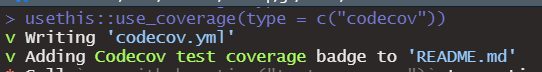
\includegraphics{images/test-coverage/addbadge.png}
  \item
    Or should give you a message in the console telling you to copy and paste some lines in the README. 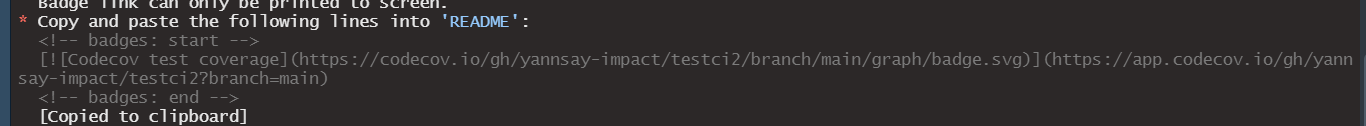
\includegraphics{images/test-coverage/copybadge.png}
  \item
    If nothing happen, you can add the line directly following the syntax or remove the \textbf{codecov.yml} from the project folder and run \texttt{usethis::use\_coverage("codecov")} again.
  \end{itemize}
\item
  Push!
\item
  The GitHub action will push the report to Codecov, you can see the report by clicking on the badge.

  \begin{itemize}
  \tightlist
  \item
    \textbf{Github and Codecov needs to sync for the percentage to appear}
  \end{itemize}
\end{itemize}

\hypertarget{style}{%
\chapter{Style}\label{style}}

\hypertarget{styler}{%
\section{styler}\label{styler}}

Quick how-to to set a github action for a styler each time there is push or a pull request with files that includes \emph{.{[}rR{]}}, \emph{.{[}rR{]}md}, \emph{.{[}rR{]}markdown}, \emph{.{[}rR{]}nw}. into the \textbf{main} using \texttt{r-lib} \href{https://github.com/r-lib/actions/blob/v2-branch/examples/style.yaml}{style.yaml}.

\hypertarget{prerequisite-2}{%
\section{Prerequisite}\label{prerequisite-2}}

None in particular.

\hypertarget{steps-2}{%
\section{Steps}\label{steps-2}}

\begin{itemize}
\item
  Create your package.
\item
  Try to test your package \texttt{styler::style\_pkg()}

  \begin{itemize}
  \tightlist
  \item
    While this step is not really necessary, it is to make sure your tests runs once and any further problems do not come from the tests.
  \end{itemize}
\item
  Add the check-release.yaml \texttt{usethis::use\_github\_action("style")}

  \begin{itemize}
  \tightlist
  \item
    You can change the styler::style\_pkg to \texttt{styler::style\_file} or \texttt{styler::style\_dir}.
  \end{itemize}

\begin{Shaded}
\begin{Highlighting}[]
\AttributeTok{  }\KeywordTok{{-}}\AttributeTok{ }\FunctionTok{name}\KeywordTok{:}\AttributeTok{ Style}
\AttributeTok{    }\FunctionTok{run}\KeywordTok{:}\AttributeTok{ styler::style\_pkg(filetype = c(".R", ".Rmd", ".Rmarkdown", ".Rnw"))}
\AttributeTok{    }\FunctionTok{shell}\KeywordTok{:}\AttributeTok{ Rscript \{0\}}
\end{Highlighting}
\end{Shaded}

  \begin{itemize}
  \tightlist
  \item
    More info and customisation on the \href{https://styler.r-lib.org/articles/styler.html}{package page}.\\
  \end{itemize}
\item
  Push!
\end{itemize}

\hypertarget{shiny-deploy}{%
\chapter{Shiny deploy}\label{shiny-deploy}}

\hypertarget{shiny-deploy-1}{%
\section{shiny-deploy}\label{shiny-deploy-1}}

Quick how to set a github action for a shiny deployment each time there is merge into the \textbf{main} (or \textbf{master}) branch using \texttt{r-lib} \href{https://github.com/r-lib/actions/blob/v2-branch/examples/shiny-deploy.yaml}{shiny-deploy.yaml}

\hypertarget{prerequisite-3}{%
\section{Prerequisite}\label{prerequisite-3}}

Make sure you have the rsconnect information.

\begin{itemize}
\tightlist
\item
  \url{https://shiny.rstudio.com/articles/shinyapps.html}
\end{itemize}

\hypertarget{steps-3}{%
\section{Steps}\label{steps-3}}

\begin{itemize}
\item
  Create your app using \texttt{renv} (The yaml use assume \texttt{renv} is used).

  \begin{itemize}
  \tightlist
  \item
    \emph{It is probably also a best practice to use renv.}
  \end{itemize}
\item
  Try to deploy your app (either with the publish/redeploy button) or \texttt{rsconnect::deployApp()}

  \begin{itemize}
  \tightlist
  \item
    While this step is not really necessary, it is to make sure your app runs once and any further problems do not come from the app itself.
  \end{itemize}
\item
  Add a description \texttt{usethis::use\_description(check\_name\ =\ F)}.

  \begin{itemize}
  \tightlist
  \item
    \emph{\texttt{check\_name\ =\ F} to avoid checking name valid for CRAN.}
  \end{itemize}
\item
  Add the shiny-deploy.yaml \texttt{usethis::use\_github\_action("shiny-deploy.yaml")}
\item
  Edit the shiny-deploy.yaml, especially the following part.

  \begin{itemize}
  \tightlist
  \item
    You can either fill in for the APPNAME, ACCOUNT, SERVER.
  \end{itemize}

\begin{Shaded}
\begin{Highlighting}[]
\AttributeTok{  }\KeywordTok{{-}}\AttributeTok{ }\FunctionTok{name}\KeywordTok{:}\AttributeTok{ Authorize and deploy app}
\AttributeTok{    }\FunctionTok{env}\KeywordTok{:}\AttributeTok{ }
\CommentTok{      \# Provide your app name, account name, and server to be deployed below}
\AttributeTok{      }\FunctionTok{APPNAME}\KeywordTok{:}\AttributeTok{ your{-}app{-}name}
\AttributeTok{      }\FunctionTok{ACCOUNT}\KeywordTok{:}\AttributeTok{ your{-}account{-}name}
\AttributeTok{      }\FunctionTok{SERVER}\KeywordTok{:}\AttributeTok{ shinyapps.io}\CommentTok{ \# server to deploy}
\FunctionTok{    run}\KeywordTok{: }\CharTok{|}
\NormalTok{      rsconnect::setAccountInfo("$\{\{ secrets.RSCONNECT\_USER \}\}", "$\{\{ secrets.RSCONNECT\_TOKEN \}\}", "$\{\{ secrets.RSCONNECT\_SECRET \}\}")}
\NormalTok{      rsconnect::deployApp(appName = "$\{\{ env.APPNAME \}\}", account = "$\{\{ env.ACCOUNT \}\}", server = "$\{\{ env.SERVER \}\}")}
\AttributeTok{    }\FunctionTok{shell}\KeywordTok{:}\AttributeTok{ Rscript \{0\}}
\end{Highlighting}
\end{Shaded}

  \begin{itemize}
  \tightlist
  \item
    Or you can remove the \texttt{env} block and change the \texttt{rsconnect::deployApp} call.
  \end{itemize}

\begin{Shaded}
\begin{Highlighting}[]
\AttributeTok{  }\KeywordTok{{-}}\AttributeTok{ }\FunctionTok{name}\KeywordTok{:}\AttributeTok{ Authorize and deploy app}
\FunctionTok{    run}\KeywordTok{: }\CharTok{|}
\NormalTok{      rsconnect::setAccountInfo("$\{\{ secrets.RSCONNECT\_USER \}\}", "$\{\{ secrets.RSCONNECT\_TOKEN \}\}", "$\{\{ secrets.RSCONNECT\_SECRET \}\}")}
\NormalTok{      rsconnect::deployApp()}
\AttributeTok{    }\FunctionTok{shell}\KeywordTok{:}\AttributeTok{ Rscript \{0\}}
\end{Highlighting}
\end{Shaded}
\item
  Add 3 secrets in the repository to store you account, token and secret (see prerequisite). They should have those names

  \begin{itemize}
  \tightlist
  \item
    \texttt{RSCONNECT\_USER}, \texttt{RSCONNECT\_TOKEN}, and secret \texttt{RSCONNECT\_SECRET}
  \item
    You can follow these \href{https://docs.github.com/en/actions/security-guides/encrypted-secrets\#creating-encrypted-secrets-for-a-repository}{guides} if needed
  \end{itemize}
\item
  Link the shiny app folder to the github repo (add the remote and origin) (if you have not done it already).
\item
  Push!
\end{itemize}

  \bibliography{book.bib,packages.bib}

\end{document}
